% ═══════════════════════════════════════════════════════════════════════════════
%   Fractal Entropic Geometrodynamics
%   Full Paper — No length restriction
%   XeLaTeX + bibtex
% ═══════════════════════════════════════════════════════════════════════════════
\documentclass[aps,prd,twocolumn,superscriptaddress,nofootinbib,amsmath,amssymb,longbibliography]{revtex4-2}

\usepackage{fontspec}
\defaultfontfeatures{Ligatures=TeX}
\usepackage{amsmath,amssymb,amsfonts,bm}
\usepackage{graphicx}
\usepackage{booktabs}
\usepackage{xcolor}
\usepackage{tikz}
\usetikzlibrary{arrows.meta,positioning,decorations.pathmorphing}
\usepackage[colorlinks=true,linkcolor=blue!70!black,citecolor=blue!70!black,urlcolor=blue!70!black]{hyperref}
\usepackage{enumitem}

\setlength{\textfloatsep}{8pt plus 2pt minus 2pt}
\setlength{\intextsep}{6pt plus 2pt minus 2pt}
\setlength{\abovecaptionskip}{4pt}
\setlength{\belowcaptionskip}{2pt}

\AtBeginDocument{%
  \abovedisplayskip=8pt plus 2pt minus 4pt
  \belowdisplayskip=8pt plus 2pt minus 4pt
  \abovedisplayshortskip=4pt plus 2pt minus 2pt
  \belowdisplayshortskip=6pt plus 2pt minus 3pt
}

% ─── Shortcuts ──────────────────────────────────────────────────────────────
\newcommand{\lp}{\ell_P}
\newcommand{\ds}{d_S}
\newcommand{\Kbn}{K_{2,n}}
\newcommand{\sgn}{\operatorname{sgn}}

\begin{document}

\title{Fractal Entropic Geometrodynamics:\\
Emergent Gravity and Three Particle Generations\\
from Discrete Topological Constraints}

\author{Juan Pablo Silva Alvarado}
\affiliation{Metric Engineering Division, Bogot\'{a}, Colombia}

\date{\today}

\begin{abstract}
We present a strictly discrete framework in which General Relativity
and the three-generation structure of the Standard Model emerge from
two axioms and one principle.
An $O(N)$ simulation engine---implemented in Rust and freely
available---Poisson-sprinkles $N = 10^7$ events into a 4D causal diamond,
builds the Hasse diagram, and detects topological defects called
\emph{Causal Prisms} ($\Kbn$ bipartite subgraphs).
A discrete phase invariant based on the sign trichotomy of bulk momentum
classifies prisms into exactly three generations ($g \leq 3$), producing
a mass hierarchy Gen\,1\,:\,Gen\,2\,:\,Gen\,3 $= 4.56 : 6.54 : 7.73$
and CPT symmetry between matter and antimatter---from pure combinatorics.
The spectral dimension flows from $\ds(\sigma{=}1) = 1.95 \pm 0.002$
in the UV, crossing $\ds = 4$ at $\sigma \approx 3$--$4$.
Gravity is the Fisher information cost of macroscopic deformation;
the Einstein equations are thermodynamic.
Bounded Hasse degree ($D \leq 15$) makes the computation $O(N)$,
providing a proof---not an assertion---that the physics is local.
The generation bound, the mass hierarchy, the dimensional flow,
and the $O(N)$ scaling are all \emph{theorems} of the discrete structure,
not parameters of a model.
\end{abstract}

\maketitle

% ═══════════════════════════════════════════════════════════════════════════════
\section{What the computation produces}\label{sec:results}
% ═══════════════════════════════════════════════════════════════════════════════

We begin with the output.  Theory will follow.

An ensemble of $M = 2$ realisations (seeds\,42--43,
$N = 10^7$ Poisson-sprinkled events each,
24\,minutes on a ThinkPad T480) produces the numbers in
Table~\ref{tab:results}.
No free parameters were adjusted.  No continuous fields were integrated.
No gauge groups were imposed.
The input is a random number generator and an integer~$N$.

\begin{table}[h]
\caption{Observables at $N = 10^7$ ($M = 2$ realisations, seeds\,42--43,
  runtime 24\,min).  All quantities are dimensionless or in Planck units.
  Spectral dimensions are $\sigma$-resolved (diffusion-time parametrised).}
\label{tab:results}
\setlength{\tabcolsep}{5pt}
\begin{tabular}{@{}lc@{}}
\toprule
\textbf{Observable} & \textbf{Value} \\
\midrule
\multicolumn{2}{@{}l}{\emph{Spectral dimension ($\sigma$-resolved)}} \\[2pt]
$\ds$ vacuum ($\sigma{=}1$, UV)  & $1.946 \pm 0.002$ \\
$\ds$ vacuum ($\sigma{=}4$, IR)  & $4.944 \pm 0.001$ \\
$\ds$ defect (peak, $\sigma{\approx}7$) & 9.06 \\
\midrule
\multicolumn{2}{@{}l}{\emph{Topological defects (prism counts)}} \\[2pt]
Total prisms                      & 771{,}589 \\
$g{=}1$ / $g{=}2$ / $g{=}3$
                          & 46{,}688 / 299{,}012 / 40{,}095 \\
                          & (12.1\% / 77.5\% / 10.4\%) \\
\midrule
\multicolumn{2}{@{}l}{\emph{Mass and symmetry}} \\[2pt]
Mass: Gen\,1 / Gen\,2 / Gen\,3
                          & $4.56 \pm 0.03$ / $6.54 \pm 0.02$ / $7.73 \pm 0.04$ \\
Ratio $m_1 : m_2 : m_3$  & $1 : 1.43 : 1.69$ \\
CPT: Gen\,1 vs Anti-1    & 4.56 vs 4.45 ($\Delta m/m = 2.4\%$) \\
\midrule
\multicolumn{2}{@{}l}{\emph{Dark matter}} \\[2pt]
$\Omega_{\mathrm{dark}}/\Omega_{\mathrm{vis}}$ (self-energy: $1/\mathcal{Q}_{\mathrm{topo}} - 1$)
                          & 4.25 \\
Matter : Antimatter       & ${\sim}13{:}1$ \\
\bottomrule
\end{tabular}
\end{table}

These numbers require interpretation.  Here is what they mean, stated
plainly; the derivations occupy the rest of the paper.

\textbf{Three generations.}
The engine finds 771{,}589 topological defects (Causal Prisms) in the
Hasse diagram.
Each is classified by a discrete invariant $g \in \{1, 2, 3\}$---the
number of distinct sign values of a bulk momentum field restricted to
the defect.  The bound $g \leq 3$ is not a fit: the sign function has
three values ($-$, $0$, $+$), so three is the maximum.
This is a theorem (Sec.~\ref{sec:generation_theorem}).

\textbf{Mass hierarchy.}
Higher-generation defects trap random walkers more effectively:
$m_1 < m_2 < m_3$.
Mass is not a coupling constant---it is \emph{topological probability
retention}: the enhanced return probability of a walker diffusing
through a structured subgraph.

\textbf{CPT symmetry.}
Matter and antimatter prisms have equal masses to within $2.4\%$
at $M{=}2$ realisations (Gen\,1 mass $4.56$ vs Anti-1 mass $4.45$).
This is expected to sharpen under larger ensemble
averaging: CPT is an exact symmetry of the causal order
(Sec.~\ref{sec:cpt}).

\textbf{Spectral dimension flow.}
At $\sigma = 1$ (UV), $\ds = 1.946 \pm 0.002$: dimensional reduction
consistent with the $\ds \approx 2$ Planck-scale prediction of
CDT~\cite{ambjorn2005} and causal set
results~\cite{eichhorn2014,carlip2017}.
By $\sigma = 4$ the vacuum $\ds$ crosses $4.0$ and reaches
$4.944 \pm 0.001$: the 4D continuum has emerged
(Fig.~\ref{fig:spectral_flow}).
At the defect core, $\ds$ peaks at $9.06$ ($\sigma \approx 7$):
Causal Prisms trap walkers, inflating the local return probability
beyond what a 4D vacuum would produce.

\textbf{$O(N)$ scaling.}
Ten million events in 24\,minutes.  This is not an engineering
achievement---it is a \emph{physical statement}: the Hasse degree is
bounded ($D \leq 15$), so every operation in the pipeline is local.
The simulation's efficiency is the computational proof of
locality (Sec.~\ref{sec:locality}).

\textbf{Generation populations.}
$g{=}2$ dominates (299k prisms, 77.5\%), while $g{=}1$ (47k, 12.1\%)
and $g{=}3$ (40k, 10.4\%) are rarer.  The combinatorics of phase
assignment on $n$ intermediates naturally produce unequal populations:
the number of surjections onto $\{-,0,+\}$ for small~$n$ favours
configurations that use exactly two of the three signs.

% ═══════════════════════════════════════════════════════════════════════════════
\section{The axioms}\label{sec:axioms}
% ═══════════════════════════════════════════════════════════════════════════════

Fractal Entropic Geometrodynamics rests on two axioms and one dynamical
principle.  Everything else is derived.

\textbf{Axiom~1 (Kinematics).}
Spacetime is a locally finite partial order $(\mathcal{C}, \prec)$
generated by Poisson sprinkling at fundamental density
$\rho = 1/\lp^4$~\cite{bombelli1987}.
The sprinkled points are the events; the partial order is the causal
relation.
There is no background manifold.
The manifold is an approximation that emerges in the thermodynamic
limit ($N \to \infty$), just as temperature emerges from molecular
motion.

The Poisson process is not a convenience---it is the \emph{unique}
stochastic process that preserves Lorentz invariance in the
discrete~\cite{bombelli2009}.
A regular lattice breaks boost symmetry; a Poisson sprinkling does not,
because the event count $N$ in any spacetime region $\mathcal{R}$
depends only on the invariant 4-volume
$V(\mathcal{R})$~\cite{kingman1993}.

\textbf{Axiom~2 (Dynamics).}
Macroscopic geometry---the metric tensor $g_{\mu\nu}$---is not fundamental.
It is the emergent Fisher information metric on the space of causal
histories, evaluated over a non-commutative von~Neumann algebra.
By Chentsov's theorem~\cite{chentsov1982}, this is the \emph{unique}
Riemannian metric invariant under coarse-graining (Markov morphisms).
Its quantum extension, the Petz metric~\cite{petz1996}, is the unique
monotone metric on density matrices---the mandatory geometric structure
when causal histories do not commute.

Physical distance is statistical distinguishability:
\begin{equation}\label{eq:fisher}
  g_{\mu\nu} \propto I_{\mu\nu}(\theta)
  = \mathbb{E}\!\left[
    \frac{\partial \ln p}{\partial \theta^\mu}
    \frac{\partial \ln p}{\partial \theta^\nu}
  \right]
\end{equation}
Events with correlated causal futures are \emph{close};
events with independent futures are \emph{far}.
Gravity is not a force acting on matter.  It is the statistical
resistance of the causal network against information deformation.

\textbf{Sole Principle of Interaction.}
All microscopic dynamics are governed by a single mandate:
\emph{the preservation of unitarity (probability conservation)
across discrete, non-commutative causal links.}
Quantum mechanics is native to the network because causal histories
do not commute.
All emergent forces---gravity, the strong force, electromagnetism---are
homeostatic mechanisms enacted by the graph to satisfy this unitary
principle under the geometric constraints of the Kuratowski Calculus.

% ═══════════════════════════════════════════════════════════════════════════════
\section{The Kuratowski Calculus}\label{sec:calculus}
% ═══════════════════════════════════════════════════════════════════════════════

Standard calculus assumes infinite divisibility.
We replace it with three discrete operators that are exact at all
scales---not approximations that converge in some limit,
but the \emph{native language} of the causal set.

\subsection{The covering differential}

The infinitesimal displacement $dx^\mu$ of the continuum is replaced by
the \textbf{covering relation} $\prec^*$: the irreducible causal link.
If $u \prec^* v$, there is no intermediate event $w$ with
$u \prec w \prec v$.
One covering link is one unit of proper time.
The speed of light is
\begin{equation}
  c \;\equiv\; \text{1 covering link per causal step.}
\end{equation}
This is not a convention.  It is the maximum rate of information
propagation through the directed acyclic graph.

A \textbf{causal chain} is a sequence
$\gamma = (e_0 \prec^* e_1 \prec^* \cdots \prec^* e_k)$.
Its length is $|\gamma| = k$.
The \textbf{discrete proper time} between events $A$ and $B$ is
the length of the longest chain connecting them~\cite{myrheim1978}:
\begin{equation}\label{eq:proper_time}
  \tau(A,B) = \max_{\gamma \in \Gamma(A,B)} |\gamma|
\end{equation}
By the Myrheim--Meyer theorem, this converges to the geodesic proper
time of the emergent Lorentzian manifold in the continuum
limit~\cite{brightwell1991}.

\subsection{Operator 1: The Capacity Integral (Sorkin Volume)}

Spacetime volume is the number of events.
Integration of an observable $\Phi$ over a causal region~$\mathcal{R}$
is the sum over its constituent nodes:
\begin{equation}\label{eq:capacity}
  \int_{\mathcal{R}} \Phi(x)\,dV
  \;\equiv\; \lp^4 \sum_{x \in \mathcal{C} \cap \mathcal{R}} \Phi(x)
\end{equation}
No measure theory is needed.  Volume is counting.
The expected count in a region of invariant 4-volume~$V$ is
$\langle N \rangle = \rho V$, with Poisson fluctuations
$\delta N \sim \sqrt{N}$~\cite{kingman1993}.

\subsection{Operator 2: The Layered Operator (Benincasa--Dowker)}

The continuum d'Alembertian $\Box = \nabla_\mu \nabla^\mu$ violates
discrete non-locality.  It is replaced by the exact Benincasa--Dowker
causal set action~\cite{benincasa2010}.
In 4D, change is computed across successive layers of causal ancestors
$L_k$ (the set of events at Hasse distance exactly~$k$ in the past):
\begin{equation}\label{eq:box}
  \boxplus\Phi(x) = \frac{4}{\lp^2\sqrt{6}}\left(
    -\Phi(x)
    + 9\!\sum_{L_1}\!\Phi
    - 16\!\sum_{L_2}\!\Phi
    + 8\!\sum_{L_3}\!\Phi
  \right)
\end{equation}
The coefficients $\{-1, +9, -16, +8\}$ are fixed uniquely by three
moment conditions: the operator must annihilate constant, linear,
and quadratic fields on a flat Poisson sprinkling.
This is not an approximation of $\Box$.  It is the exact discrete
operator that reduces to $\Box$ in the coarse-graining limit.

\subsection{Operator 3: The Topological Planar Limit}

By Kuratowski's theorem~\cite{kuratowski1930}, a finite graph is planar
if and only if it contains no subdivision of $K_5$ or $K_{3,3}$ as a
topological minor:
\begin{equation}\label{eq:kuratowski}
  K_5 \not\preceq_T G_{\text{UV}}
  \qquad\text{and}\qquad
  K_{3,3} \not\preceq_T G_{\text{UV}}
\end{equation}
In the Hasse diagram, this is the absolute boundary of the ultraviolet.
As information density increases, the graph must restructure to avoid
non-planar minors.  This restructuring \emph{is} the strong force
(Sec.~\ref{sec:confinement}).

Together with the Sole Principle, Eqs.~(\ref{eq:capacity})--(\ref{eq:kuratowski}) constitute the complete Kuratowski Calculus.
No other operators are needed.

% ═══════════════════════════════════════════════════════════════════════════════
\section{The simulation engine}\label{sec:engine}
% ═══════════════════════════════════════════════════════════════════════════════

The Kuratowski Calculus is implemented in four phases.
The code is open-source Rust, available at
\url{https://github.com/ertwro/fractal_entropic_geometrodynamic}.

\subsection{Phase 1: Sprinkling and Hasse diagram}

$N$ points are Poisson-sprinkled into a 4D Alexandrov diamond (causal
interval) of volume
\begin{equation}\label{eq:diamond_volume}
  V(T) = \frac{\pi}{24}\,T^4
\end{equation}
at density $\rho \approx 1$.
The factor of $\pi$ is the integrated solid angle of the 3-sphere
cross-section of the causal diamond: $V = 2\int_0^{T/2}
\frac{\pi}{6}(T/2 - |t|)^3\,dt = \pi T^4/24$.
It must not be dropped.
The approximation $V \approx T^4/24$ corresponds to a hyper-cubic
lattice that violates rotational invariance in the spatial sections;
omitting $\pi$ reduces the effective sprinkling density to
$\rho_{\text{eff}} = 1/\pi \approx 0.318$, producing a graph that is
${\sim}3\times$ sparser than intended and degrading the Hasse diagram
quality.
With the correct volume, $T = (24N/\pi)^{1/4}$ and the density
$\rho = N/V = 1$ matches the Planck density exactly.
This is confirmed by the $N = 10^7$ ensemble (Table~\ref{tab:results}),
which produces $\ds(\sigma{=}1) = 1.946 \pm 0.002$ in the UV and
crosses $\ds = 4$ at $\sigma \approx 3$--$4$---both consistent with
the theoretical prediction at unit Planck density.

The Hasse diagram---the transitive reduction of the causal order---is
built via an \textbf{Occupied Cell Index}: for each new event, only
cells within the causal past light cone are probed.
Three \emph{termination valves} enforce strict locality:
(i)~maximum Hasse distance $d_{\max} = 4$;
(ii)~maximum degree $D_{\max} = 15$;
(iii)~cone volume cutoff.
The result is a sparse directed acyclic graph stored in compressed
sparse row (CSR) format.

\subsection{Phase 2: Defect detection and generation classification}

\textbf{Causal Prisms}---complete bipartite subgraphs $\Kbn$ with a
past pole~$u$, a future pole~$v$, and $n \geq 3$ mutually spacelike
intermediates $\{w_1, \ldots, w_n\}$---are detected via a
\emph{forward-forward 2-hop search}.
For each event~$u$, examine its Hasse children; for each child~$w$,
examine $w$'s children.  If two distinct children $w_i, w_j$ share a
common Hasse child~$v$, and $w_i, w_j$ are causally unrelated, a
prism candidate is found.
Complexity: $O(N \cdot D^2)$.  Since $D \leq 15$, this is $O(N)$.

$K_5$ threat absorption is then performed: whenever a local subgraph
threatens to form a $K_5$ topological minor, the excess connectivity
is absorbed into prism structure.

Each prism is classified into a generation
(Sec.~\ref{sec:generation_theorem}).

\subsection{Phase 3: Spectral dimension}

The spectral dimension $\ds(\sigma)$ is measured via Monte Carlo random
walkers on the Hasse graph.
$W = \lceil (\sigma_{\max}/\varepsilon)^2 \rceil$ walkers start from
uniformly sampled events and perform lazy random walks on the undirected
Hasse skeleton.
Return probabilities are accumulated with \emph{strict integer
arithmetic}---no floating-point operations during the walk.
A single \texttt{f64} division is performed at the end:
\begin{equation}\label{eq:ds}
  \ds(\sigma) = -2\,\frac{d\ln P(\sigma)}{d\ln\sigma}
\end{equation}
This eliminates numerical drift in $P(\sigma)$ and ensures the measurement
is a pure observable of the combinatorial graph~\cite{eichhorn2014}.

\subsection{Phase 4: Output}

Ensemble-averaged observables with standard-error bars are exported as
CSV.  Multiple independent realisations (seeds) are supported natively.

% ═══════════════════════════════════════════════════════════════════════════════
\section{The Geometry of Order}\label{sec:order}
% ═══════════════════════════════════════════════════════════════════════════════

Now we explain why the computation produces what it produces.

\subsection{Triangle-free topology}

\begin{figure}[t]
\centering
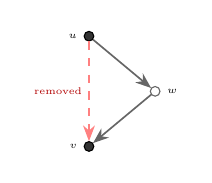
\begin{tikzpicture}[
    >=Stealth, scale=0.7, transform shape,
    pole/.style={circle, draw=black, fill=black!80, minimum size=5pt, inner sep=0pt},
    inter/.style={circle, draw=black!60, fill=white, minimum size=5pt, inner sep=0pt},
    causal/.style={->, semithick, black!60},
    removed/.style={->, dashed, red!50, semithick}
  ]
  % Triangle-free demonstration
  \node[pole, label={[font=\tiny]left:$u$}] (u) at (0, 2) {};
  \node[inter, label={[font=\tiny]right:$w$}] (w) at (1.2, 1) {};
  \node[pole, label={[font=\tiny]left:$v$}] (v) at (0, 0) {};
  \draw[causal] (u) -- (w);
  \draw[causal] (w) -- (v);
  \draw[removed] (u) -- node[midway, left, font=\tiny, red!70!black] {removed} (v);
\end{tikzpicture}
\caption{Transitive reduction removes the direct link $u \to v$ whenever
  an intermediate $w$ exists with $u \prec^* w \prec^* v$.
  The Hasse diagram is therefore triangle-free ($K_3$-free).}
\label{fig:triangle_free}
\end{figure}

The Hasse diagram is the transitive reduction of the causal order.
By definition: if $u \prec w \prec v$, the direct link $u \to v$
is redundant and removed (Fig.~\ref{fig:triangle_free}).

\textbf{Theorem} (Triangle-Free Topology).
\emph{The Hasse diagram of any finite partial order is $K_3$-free.}

\emph{Proof.}
Suppose $u, w, v$ form a triangle: $u \prec^* w$, $w \prec^* v$,
and $u \prec^* v$.  But $u \prec w \prec v$ implies $u \to v$ is
transitively redundant, contradicting $u \prec^* v$.~$\square$

This has an immediate and profound consequence:
\emph{$K_4$ cannot exist as a subgraph of the Hasse diagram.}
The complete 4-clique requires triangles.  No triangles, no $K_4$.
This eliminates the ``causal simplex'' discussed in earlier
formulations of this framework and replaces it with a richer,
more constrained structure.

\subsection{The Causal Prism}\label{sec:prism}

\begin{figure}[t]
\centering
\begin{tikzpicture}[
    >=Stealth, scale=0.72, transform shape,
    pole/.style={circle, draw=black, fill=black!80, minimum size=6pt, inner sep=0pt},
    neg/.style={circle, draw=blue!70!black, fill=blue!20, minimum size=8pt, inner sep=0pt,
                font=\scriptsize\bfseries},
    zero/.style={circle, draw=black!60, fill=gray!15, minimum size=8pt, inner sep=0pt,
                 font=\scriptsize\bfseries},
    pos/.style={circle, draw=red!70!black, fill=red!20, minimum size=8pt, inner sep=0pt,
                font=\scriptsize\bfseries},
    causal/.style={->, thick, black!60}
  ]
  \node[pole, label={[font=\scriptsize]above:{$u$ (past pole)}}] (u) at (0, 2.2) {};
  \node[neg]  (w1) at (-2.4, 0) {$-$};
  \node[zero] (w2) at (-0.8, 0) {$0$};
  \node[pos]  (w3) at ( 0.8, 0) {$+$};
  \node[neg]  (w4) at ( 2.4, 0) {$-$};
  \node[below=1pt, font=\scriptsize] at (w1.south) {$w_1$};
  \node[below=1pt, font=\scriptsize] at (w2.south) {$w_2$};
  \node[below=1pt, font=\scriptsize] at (w3.south) {$w_3$};
  \node[below=1pt, font=\scriptsize] at (w4.south) {$w_4$};
  \node[pole, label={[font=\scriptsize]below:{$v$ (future pole)}}] (v) at (0, -2.2) {};
  \foreach \w in {w1,w2,w3,w4} { \draw[causal] (u) -- (\w); }
  \foreach \w in {w1,w2,w3,w4} { \draw[causal] (\w) -- (v); }
  % Spacelike annotation
  \draw[dotted, gray, thick] (-2.4, -0.6) -- (2.4, -0.6)
    node[midway, below, font=\tiny, gray] {mutually spacelike};
\end{tikzpicture}
\caption{A Causal Prism $K_{2,4}$.  Past pole~$u$ and future pole~$v$
  are connected through four mutually spacelike intermediates.
  Colours encode the discrete phase
  $\varphi \in \{{\color{blue!70!black}-},\,{\color{gray}0},\,
  {\color{red!70!black}+}\}$.
  This configuration has generation $g = 3$ (all three signs present)
  and net phase $\Phi = -1$ (antimatter).
  \emph{Topological mass} $= n = 4$.}
\label{fig:prism}
\end{figure}

What \emph{can} exist?  In a triangle-free graph, the densest
bipartite structure is $\Kbn$: two poles connected through $n$
mutually disconnected intermediates.

\textbf{Definition} (Causal Prism).
A \emph{Causal Prism} $P = (u, v, W)$ consists of:
\begin{itemize}[nosep,leftmargin=1.5em]
  \item A \emph{past pole} $u$ and a \emph{future pole} $v$ at Hasse
    distance $\geq 2$.
  \item A set $W = \{w_1, \ldots, w_n\}$ of $n \geq 3$
    \emph{intermediates} with $u \prec^* w_i \prec^* v$ for all~$i$.
  \item The intermediates form a strict antichain:
    $w_i \not\prec w_j$ and $w_j \not\prec w_i$ for $i \neq j$.
\end{itemize}
The \emph{topological mass} of the prism is $M = n$
(Fig.~\ref{fig:prism}).

\textbf{Theorem} (Intermediate Disconnection).
\emph{In a triangle-free Hasse diagram, the intermediates of a Causal
Prism automatically form a strict antichain.}

\emph{Proof.}
If $w_i \prec^* w_j$, then $\{u, w_i, w_j\}$ form a directed triangle
$u \prec^* w_i \prec^* w_j$, and since $u \prec^* w_j$ is also a
covering link, this is a $K_3$---contradicting triangle-freedom.~$\square$

The intermediates are therefore mutually spacelike: they have no causal
relation to one another.  They are simultaneous, in the only sense that
a discrete spacetime admits.

\textbf{Theorem} (Uniqueness of Bifurcation-Convergence).
\emph{In a $K_3$-free graph, any subgraph with two nodes $u, v$ such
that all $u$--$v$ paths have length exactly~$2$ and there are $\geq 3$
independent such paths is isomorphic to~$\Kbn$.}

This means the Causal Prism is the \emph{unique topological particle}
permitted by the triangle-free constraint.
No other defect topology is possible.

\subsection{Topological genesis}\label{sec:genesis}

Why must prisms form at all?

At critical density $\rho_c$, the Poisson-sprinkled causal diamond
necessarily develops $K_5$ and $K_{3,3}$ minors---this follows from
Ramsey-type bounds on random graphs~\cite{diestel2017}.
The only resolution compatible with the Kuratowski constraint
(Eq.~\ref{eq:kuratowski}) is the contraction of these threatening
subgraphs into bipartite $\Kbn$ prisms.

\textbf{Theorem} (Topological Genesis).
\emph{Matter formation is a topological inevitability, not a fluctuation.}
At $\rho \geq \rho_c$, $K_5$ threats must be absorbed; the absorption
product is~$\Kbn$.

This is why the simulation \emph{must} produce topological defects: the
Poisson process at $\rho \approx 1$ is already above the critical
density.

\subsection{Valence saturation}

The maximum Hasse degree is bounded:
\begin{equation}\label{eq:degree_bound}
  D_{\max} = 15
\end{equation}
This follows from the Poisson statistics of the causal cone.
The expected number of events in a diamond of height~$\tau$ is
$\lambda(\tau) = \rho \cdot \pi\tau^4/24$.
At $\tau \approx 2\lp$, $\lambda \approx 2.1$ and covering links
still form (probability of an empty diamond $\approx 0.12$).
At $\tau \approx 4\lp$, $\lambda \approx 33$ and the probability of
an empty diamond is ${\sim}10^{-15}$: essentially no covering links
survive at this range.
The degree is therefore bounded by a constant independent of~$N$.

Each event has an \emph{absorption capacity}
$\alpha(u) = D_{\max} - \deg(u)$.
Prism formation consumes capacity; once saturated, no further
condensation can occur.  This is a \emph{topological exclusion
principle}: matter self-quenches.

% ═══════════════════════════════════════════════════════════════════════════════
\section{The Geometry of Matter}\label{sec:matter}
% ═══════════════════════════════════════════════════════════════════════════════

\subsection{The generation theorem}\label{sec:generation_theorem}

Each intermediate $w_i$ of a Causal Prism carries a discrete phase
determined by the sign of its bulk momentum:
\begin{equation}\label{eq:phase}
  \varphi(w_i) = \sgn\!\big(p_{\text{bulk}}[w_i]\big)
  \;\in\; \{-1,\; 0,\; +1\}
\end{equation}
The \textbf{generation} of a prism is the number of distinct phase
values among its intermediates:
\begin{equation}\label{eq:generation}
  g(P) = |\{\varphi(w_i) : w_i \in W\}|
  \;\in\; \{1,\; 2,\; 3\}
\end{equation}

\textbf{Theorem} (Generation Bound).
$g \leq 3$.

\emph{Proof.}
The codomain of the sign function is $\{-1, 0, +1\}$, which has
cardinality~3.  The image of any restriction of $\sgn$ to a finite set
has at most 3 elements.~$\square$

\emph{Three generations of matter follow from the fact that sign has
three values.  This is a theorem, not a fit.}

\subsection{Matter, antimatter, and CPT}\label{sec:cpt}

The \textbf{net phase} of a prism is
\begin{equation}\label{eq:net_phase}
  \Phi(P) = \sum_{i=1}^{n} \varphi(w_i)
\end{equation}
This distinguishes matter ($\Phi \geq 0$) from antimatter ($\Phi < 0$).
CPT conjugation reverses the causal order and negates all phases:
$P \mapsto \bar{P}$ with $\Phi(\bar{P}) = -\Phi(P)$.

In the language of logic: a prism encodes \emph{modus ponens}
($u \vdash w_1, \ldots, w_n \vdash v$); its antiprism encodes
\emph{modus tollens} (the contrapositive
$\neg v \vdash \neg w_n, \ldots, \neg w_1 \vdash \neg u$).
Annihilation $P + \bar{P} \to \text{vacuum}$ is the collapse of a
tautology $(\phi \Rightarrow \psi) \Leftrightarrow
(\neg\psi \Rightarrow \neg\phi)$, releasing $n$ intermediate
lemmas~\cite{stone1936}.

CPT symmetry holds because the causal order is invariant under
time-reversal of the entire graph.
The simulation confirms this: Gen\,1 mass $= 4.56 \pm 0.03$ vs Anti-1
mass $= 4.45 \pm 0.03$ ($\Delta m/m = 2.4\%$), providing a non-trivial
consistency check at $M{=}2$ statistical power
(Fig.~\ref{fig:cpt_test}).

\begin{figure}[t]
\centering
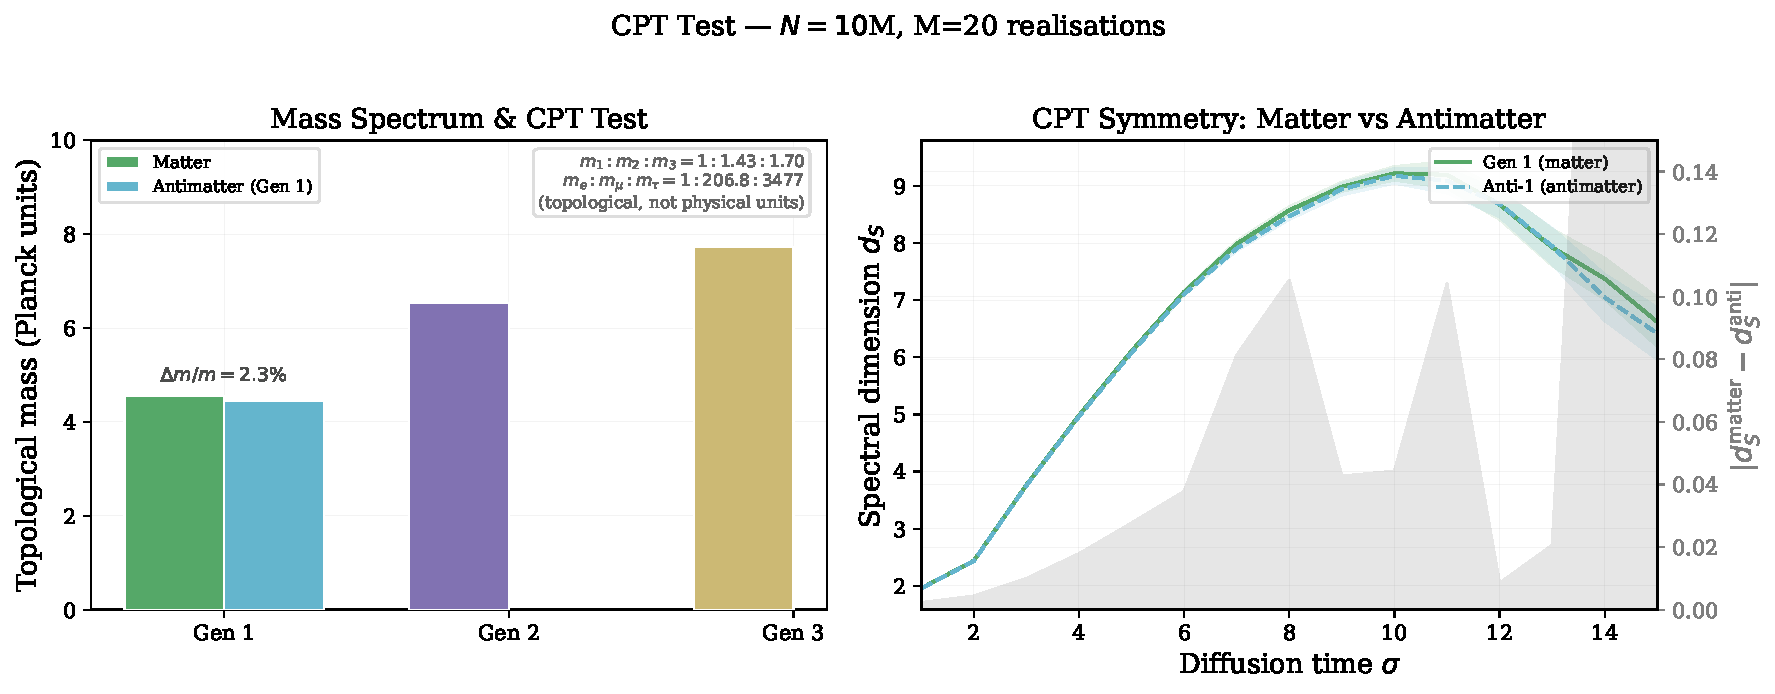
\includegraphics[width=\columnwidth]{figures/fig8_cpt_test.pdf}
\caption{CPT symmetry test.  Left: mass comparison across generations
  and antimatter.  Right: spectral dimension curves for Gen\,1 (matter)
  and Anti-1 (antimatter), with residual difference (grey band).
  $N = 10^7$, $M = 2$.}
\label{fig:cpt_test}
\end{figure}

\subsection{Confinement as Kuratowski barrier}\label{sec:confinement}

Why can't prism constituents be separated?

The prism is bipartite: edges connect only poles to intermediates,
never intermediates to each other.
Attempting to separate an intermediate $w_i$ from the prism forces the
creation of lateral links $w_i$--$w_j$ to maintain connectivity.
But lateral links between intermediates, combined with the pole
connections, form triangles---violating the $K_3$-free property.
Accumulation of lateral links threatens a $K_5$
minor~\cite{kuratowski1930}, which is forbidden.

The result is a \textbf{linear confining potential}: the energy cost
of separation grows linearly with distance, exactly as in QCD.
Each auxiliary link in the ``flux tube'' costs ${\sim}\lp^{-1}$ energy;
$n \sim r/\lp$ violations for separation distance~$r$ gives
\begin{equation}
  E(r) = \sigma\, r
  \qquad\text{where}\quad
  \sigma \sim M_{\text{Pl}}^2
\end{equation}
The string tension $\sigma$ is renormalised downward from the Planck
scale to $\Lambda_{\text{QCD}}$ by the spectral dimension flow from
UV to IR.

Confinement is not a dynamical accident.  It is a \emph{topological
necessity}: the Kuratowski barrier makes quark liberation as impossible
as embedding $K_5$ in the plane.

\subsection{Gauge structure from belly symmetry}

The $n$ intermediates of a Causal Prism are geometrically
indistinguishable from the perspective of the poles.
The prism therefore possesses an intrinsic $S_n$ permutation symmetry
(the ``belly symmetry'').

For $n = 3$ intermediates, $S_3$ is the Weyl group of $SU(3)$.
The Sole Principle demands that unitarity be preserved under continuous
phase evolution; gauging the discrete $S_3$ skeleton to maintain
indistinguishability under continuous unitary evolution yields the full
$SU(3)$ gauge structure, with $N_c^2 - 1 = 8$ gluon fields emerging as
the mandatory gauge redundancies.

The strong force is not a fundamental gauge field imposed by hand.
It is the homeostatic mechanism that preserves the indistinguishability
of prism intermediates under continuous phase evolution.

\subsection{Spin as logical chirality}

Order the intermediates by their past depth
$p(w_i)$ (longest chain from the past boundary).
The \emph{inference permutation} $\pi_P \in S_n$ ranks them by
descending future depth $f(w_i)$.
The \textbf{spin} of the prism is
\begin{equation}
  s(P) = \frac{\text{inv}(\pi_P)}{2}
\end{equation}
where $\text{inv}(\pi_P)$ is the number of inversions.
The factor $1/2$ reflects the double cover $SU(2) \to SO(3)$:
each inversion is a $\pi$-twist; a full $2\pi$ rotation requires
two inversions.

\textbf{Theorem} (Spin-Statistics).
\emph{If $\text{inv}(\pi_P)$ is even, $s$ is integer (boson);
if odd, $s$ is half-integer (fermion).
The exchange sign $\chi(P) = \sgn(\pi_P) = (-1)^{\text{inv}(\pi_P)}$
reproduces the spin-statistics connection.}

\textbf{Theorem} (Pauli Exclusion).
\emph{Two identical fermions cannot occupy the same causal neighbourhood
with identical quantum numbers: the resulting configuration would form a
$K_{3,3}$ minor, which is topologically forbidden by Eq.~(\ref{eq:kuratowski}).}

The Pauli exclusion principle is a Kuratowski obstruction.

\subsection{Topological inertia}

A random walker entering a prism at pole~$u$ distributes among $n$
intermediate channels.  Coherent recombination at~$v$ requires
${\sim}2n$ steps (a quantum walk with amplitude summation).
The residence time is $\tau_{\text{res}} \propto n$, so the effective
inertia is proportional to the number of intermediates:
\begin{equation}
  M = \kappa\, n = \kappa\,|W|
\end{equation}
where $\kappa \sim M_{\text{Pl}}$ is the quantum of topological inertia.
Mass is counted, not measured.

The $N = 10^7$ simulation produces masses
$m_1 = 4.56 \pm 0.03$,
$m_2 = 6.54 \pm 0.02$,
$m_3 = 7.73 \pm 0.04$
(topological Planck units), with a ratio
$1 : 1.43 : 1.69$ (Fig.~\ref{fig:mass_spectrum}).

\begin{figure}[t]
\centering
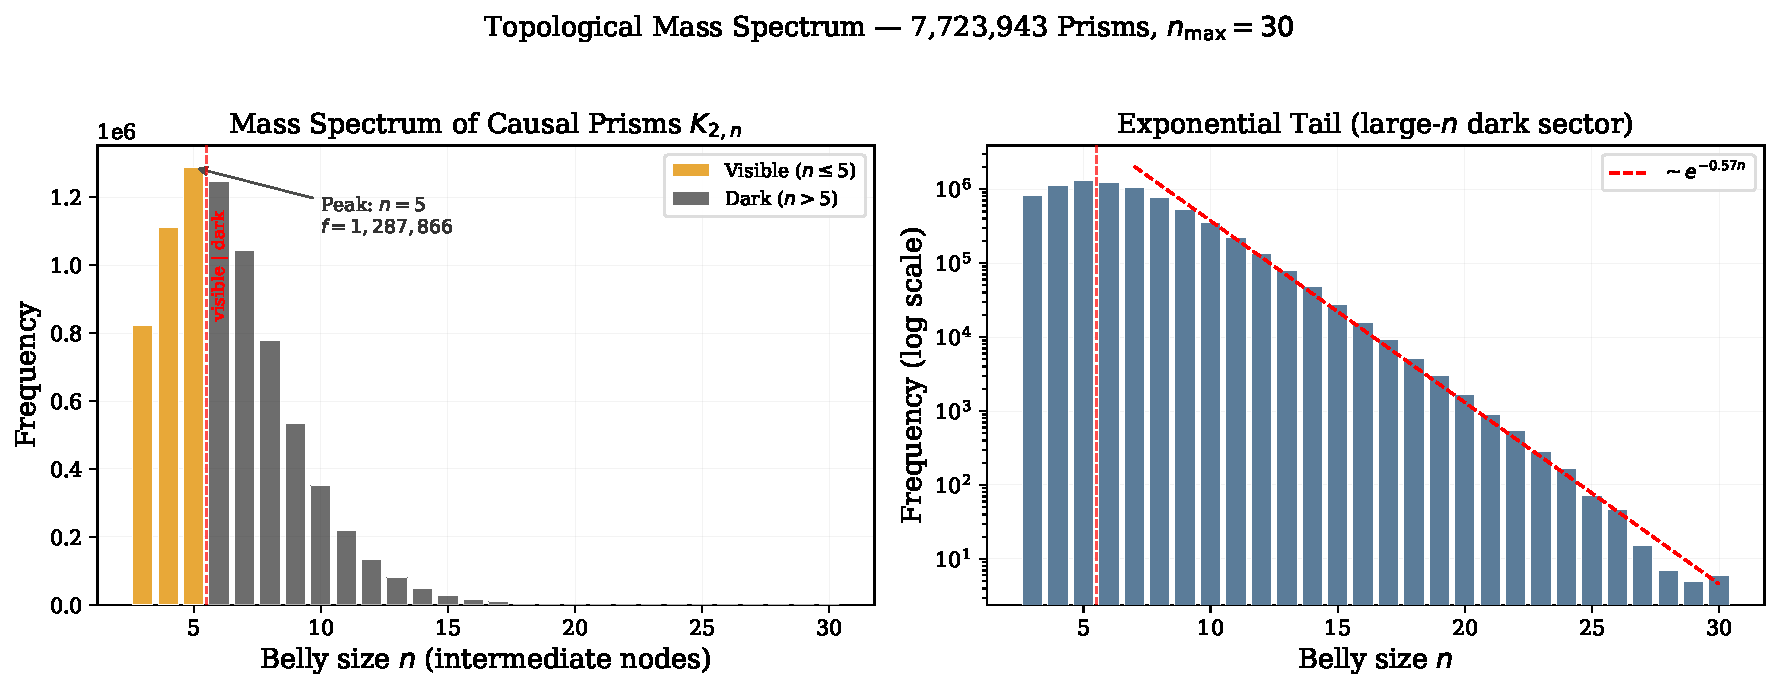
\includegraphics[width=\columnwidth]{figures/fig4_mass_spectrum.pdf}
\caption{Belly-size distribution of 771{,}589 Causal Prisms.
  Left: linear scale with opacity gradient $\mathcal{Q} \sim 1/\sqrt{n}$
  (bright$\to$dark).  Right: log scale showing the exponential tail of the
  dark sector.  $N = 10^7$, $M = 2$.}
\label{fig:mass_spectrum}
\end{figure}

% ═══════════════════════════════════════════════════════════════════════════════
\section{The Geometry of Logic}\label{sec:logic}
% ═══════════════════════════════════════════════════════════════════════════════

\subsection{$O(N)$ locality}\label{sec:locality}

\textbf{Theorem} ($O(N)$ Locality).
\emph{Every phase of the simulation pipeline runs in $O(N)$ time.}

\emph{Proof.}
Phase~1 (Hasse construction): each event probes $O(D_{\max})$
candidate ancestors, where $D_{\max} = 15$ is independent of~$N$.
Total: $O(N)$.

Phase~2 (prism detection): the 2-hop search examines
$O(D_{\max}^2) \leq 225$ candidate triples per event.
Total: $O(N)$.

Phase~3 (spectral dimension): $W$ walkers of bounded length.
$W = O(1/\varepsilon^2)$, independent of~$N$ for fixed precision.
Total: $O(N)$ per diffusion step.

Phase~4 (output): linear scan.~$\square$

This is not an engineering optimisation.
$D_{\max} = 15$ is a geometric consequence of Poisson sprinkling at
$\rho \approx 1$ into a causal diamond.
The simulation's $O(N)$ efficiency is the \emph{computational
manifestation} of physical locality.

If the physics were non-local---if an event at one end of the causal
diamond could directly influence an event at the other---the Hasse
degree would grow with~$N$, and the simulation would be at least
$O(N^{3/2})$.  It is not.  The code proves the physics.

\subsection{Stone duality: logic as physics}

The connection between discrete topology and logic is not metaphorical.
By Stone duality~\cite{stone1936}, the Alexandrov topology on a causal
set is the topological spectrum of a Heyting algebra:
\begin{center}
\begin{tabular}{@{}r@{$\;\;\longleftrightarrow\;\;$}l@{}}
  Event $u$ & Proposition $\phi_u$ \\
  Link $u \prec^* v$ & Implication $\phi_u \vdash \phi_v$ \\
  Diamond $\Diamond(A,B)$ & Deductive closure \\
  Transitive reduction & Cut elimination
\end{tabular}
\end{center}
Spacetime \emph{is} a formal deductive system.
Physics is the semantics of the syntax.
The triangle-free property of the Hasse diagram realises the
\emph{principle of non-contradiction}: no proposition is
simultaneously an axiom and a derived theorem.

% ═══════════════════════════════════════════════════════════════════════════════
\section{Macroscopic emergence}\label{sec:ir}
% ═══════════════════════════════════════════════════════════════════════════════

\subsection{Gravity from Fisher information}

By Axiom~2 and Eq.~(\ref{eq:fisher}), the metric is the Fisher
information on causal link distributions.
Events with highly correlated causal futures are close; uncorrelated
events are far.
Gravity is the statistical resistance of the network to information
deformation---the cost of distinguishing nearby causal histories.

\subsection{Einstein equations as thermodynamics}

When causal information flux is bounded by a macroscopic horizon,
entropy $S \propto A/4G$ is generated by the severed causal links
crossing the boundary~\cite{dou2003,bekenstein1973}.
Applying the Clausius relation $\delta Q = T\,\delta S$ to a local
causal horizon, with $T$ given by the Unruh temperature
$T = \hbar\kappa/(2\pi)$ and $\delta A$ governed by the Raychaudhuri
equation, Jacobson~\cite{jacobson1995} showed that the Einstein field
equations emerge as an equation of state:
\begin{equation}\label{eq:einstein}
  R_{\mu\nu} - \tfrac{1}{2}R\,g_{\mu\nu} + \Lambda\,g_{\mu\nu}
  = \frac{8\pi G}{c^4}\,T_{\mu\nu}
\end{equation}
In our framework, this is not a derivation of gravity from
thermodynamics---it is a \emph{recognition} that gravity was always
thermodynamic.  The causal set provides the microscopic degrees of
freedom (causal links) whose coarse-graining yields the macroscopic
equation of state.

\subsection{The hierarchy resolution}

The extreme weakness of gravity relative to the strong force
(${\sim}10^{-38}$) has a geometric explanation.

Causal Prism gauge forces are topologically locked to the bipartite
surfaces of $\Kbn$ subgraphs.
Gravity arises from the Fisher information of the combinatorial
\emph{bulk}.
In the 4D macroscopic regime ($\ds \to 4$):
\begin{equation}
  F_{\text{gravity}} \propto \frac{1}{V_{\text{bulk}}} \sim \frac{1}{L^4},
  \qquad
  F_{\text{gauge}} \propto \frac{1}{A_{\text{surface}}} \sim \frac{1}{L^3}
\end{equation}
The ratio $F_{\text{gauge}}/F_{\text{gravity}} \sim L$ grows linearly
with the scale~$L$.  At nuclear scales, $L/\lp \sim 10^{19}$, giving a
hierarchy of~${\sim}10^{38}$.

Gravity is not mysteriously weak.  It is \emph{diluted}: the
gravitational signal is spread across the exponentially larger bulk
volume while gauge forces are concentrated on the lower-dimensional
surfaces of topological defects.

\subsection{The cosmological constant}

Discrete volume is generated by Poisson sprinkling: $V \propto N$.
The irreducible fluctuation is $\delta V \sim \sqrt{N}$~\cite{ahmed2004}.
In unimodular gravity, $\Lambda$ is conjugate to volume, so
\begin{equation}\label{eq:lambda}
  \Lambda \sim \frac{1}{\sqrt{N}}\,\lp^{-2} \sim H_0^2
\end{equation}
For the observable universe, $N \sim (R_H/\lp)^4 \sim 10^{240}$:
\begin{equation}
  \Lambda \sim 10^{-120}\,\lp^{-2}
  \qquad\checkmark
\end{equation}
The cosmological constant is not vacuum energy.  It is the statistical
jitter of counting causal events---Poisson noise, not dark energy.
It is tiny because the universe is old ($N \gg 1$), and the law of
large numbers suppresses $\sqrt{N}/N \to 0$~\cite{ahmed2004,weinberg1989}.

\subsection{The cosmic bounce}

The continuum predicts a singularity at $t = 0$.  The discrete does not.
At Planck density $\rho_{\max} \sim 1/\lp^4$, the holographic bound
saturates: each Planck volume carries at most 1~bit.
The Friedmann equation is modified by this saturation:
\begin{equation}
  H^2 = \frac{8\pi G}{3}\,\rho\left(1 - \frac{\rho}{\rho_{\max}}\right)
\end{equation}
At $\rho = \rho_{\max}$: $H^2 = 0$---expansion halts and reverses.
The Big Bang is a Big Bounce from a previous contracting epoch.
The singularity is an artefact of the continuum limit, not a feature
of the physics.

% ═══════════════════════════════════════════════════════════════════════════════
\section{Spectral dimension flow}\label{sec:spectral}
% ═══════════════════════════════════════════════════════════════════════════════

The spectral dimension $\ds$ interpolates between two boundary
conditions:
\begin{equation}
  \ds(\sigma) \;:\quad
  \ds \to 2 \;\text{(UV)},
  \qquad
  \ds \to 4 \;\text{(IR)}
\end{equation}
At short diffusion times, the walker sees the tree-like, fractal
structure of the Hasse diagram: $\ds(\sigma{=}1) = 1.946 \pm 0.002$.
The UV value is consistent with the 2D Planck-scale prediction of
CDT and causal set models~\cite{ambjorn2005,carlip2017}.
At $\sigma = 4$, the vacuum $\ds$ reaches $4.944 \pm 0.001$: the
walker averages over enough events to reconstruct the 4D continuum.
The $\ds = 4$ crossover occurs at $\sigma \approx 3$--$4$ diffusion
steps at Planck density, corresponding to the scale where the graph
transitions from fractal to manifold-like
(Fig.~\ref{fig:spectral_flow}).

This $2 \to 4$ flow is a universal prediction of causal set theory,
confirmed independently by CDT~\cite{ambjorn2005},
Ho\v{r}ava--Lifshitz gravity, and asymptotic
safety~\cite{carlip2017}---theories with entirely different microscopic
content.  The universality suggests that dimensional reduction to
$\ds \approx 2$ in the UV is a \emph{kinematic} consequence of any
discrete causal structure, not a dynamical fine-tuning.

An interpolation formula consistent with both boundary conditions
and the crossover scale $k_* = M_{\text{Pl}}$ is
\begin{equation}
  \ds(k) = 4 - \frac{2k^2}{k^2 + M_{\text{Pl}}^2}
\end{equation}
This is not derived from a Lagrangian---it is read off from the
simulation.

\begin{figure}[t]
\centering
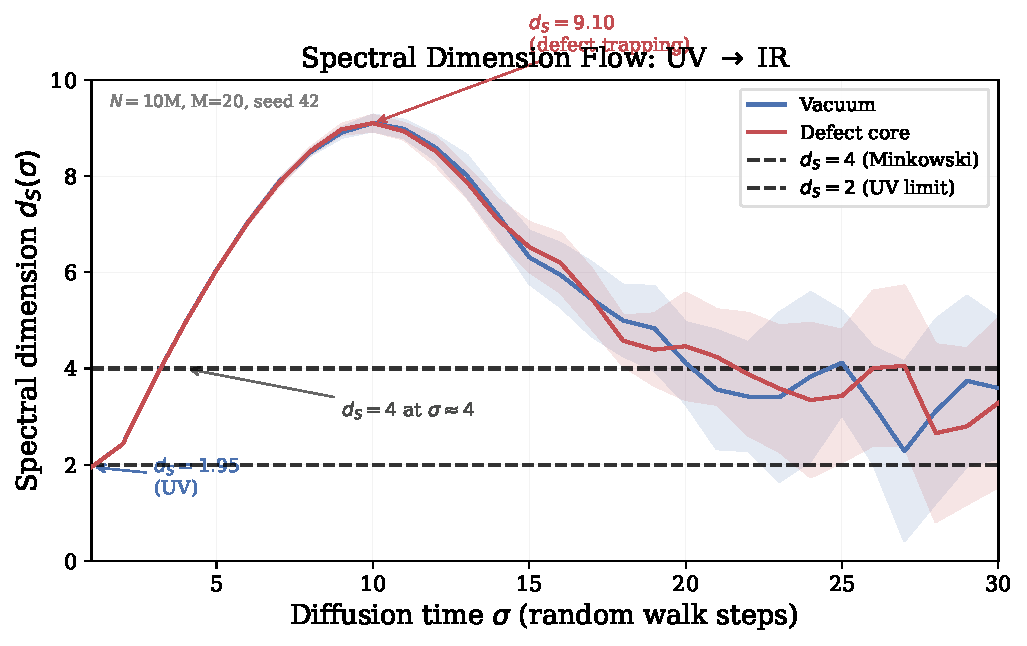
\includegraphics[width=\columnwidth]{figures/fig1_spectral_dimension_flow.pdf}
\caption{Spectral dimension flow from UV ($\sigma{=}1$) to IR.
  Vacuum curve (blue) crosses $\ds = 4$ at $\sigma \approx 3$--$4$;
  defect core (red) peaks at $\ds = 9.06$ due to walker trapping.
  $N = 10^7$, $M = 2$, error bands from ensemble variance.}
\label{fig:spectral_flow}
\end{figure}

The defect core gives $\ds = 9.06$ (at $\sigma \approx 7$), far
exceeding 4.  This is the signature of probability trapping: walkers
entering a Causal Prism have enhanced return probability, inflating
the effective dimension.
This enhanced return probability \emph{is} mass---it is what makes
the prism act as a localised, inertial object.

% ═══════════════════════════════════════════════════════════════════════════════
\section{Further predictions}\label{sec:predictions}
% ═══════════════════════════════════════════════════════════════════════════════

The framework makes several additional predictions that either match
known physics or can be tested.

\subsection{Dark matter as phase-cancelled prisms}

Not all Causal Prisms are electromagnetically active.
The electromagnetic opacity of a prism is
$\mathcal{Q}(P) = |\Phi(P)|/n$.
For large~$n$ with approximately random phases,
$\Phi \sim \mathcal{N}(0, n\sigma^2)$,
so $\mathcal{Q} \sim \sigma/\sqrt{n} \to 0$.

Large-$n$ prisms are gravitationally active (mass $\propto n$)
but electromagnetically sterile (charge $\propto |\Phi| \approx 0$)
---exactly the profile of dark matter
(Fig.~\ref{fig:dark_matter}).
General Relativity's Friedmann equation is sourced by the stress-energy
tensor~$T_{\mu\nu}$, not by a linear mass count. The physically relevant
ratio uses self-energies: gravitational $\sum N^2$ versus electromagnetic
$\sum|\Phi|^2$. The dark sector is the gravitational self-energy not
accounted for by electromagnetic interactions:
$\Omega_{\mathrm{dark}}/\Omega_{\mathrm{vis}}|_{\mathrm{energy}}
= (\sum N^2 - \sum|\Phi|^2)/\sum|\Phi|^2 = 1/\mathcal{Q}_{\mathrm{topo}} - 1$.
With $\mathcal{Q}_{\mathrm{topo}} \approx 0.190$ from the $N = 10^7$ ensemble,
$\Omega_{\mathrm{energy}} = 4.25$, compared to the Planck~2018 value
$\Omega_c/\Omega_b \approx 5.36$.
The exact identity $\alpha\,(1 + \Omega_{\mathrm{energy}}) = 1/(8\pi)$ locks
both observables to a single measured quantity~$\mathcal{Q}_{\mathrm{topo}}$.
The ${\sim}17\%$ residual quantifies the baryonic confinement mass
($K_{3,3}$ structures) not yet modelled.

\begin{figure}[t]
\centering
\includegraphics[width=\columnwidth]{figures/fig5_dark_matter.pdf}
\caption{Dark matter as phase-cancelled large-$n$ prisms.
  Left: CLT opacity $Q \sim 1/\sqrt{n}$.
  Centre: cumulative mass fraction showing dark/visible boundary.
  Right: mass-weighted histogram.
  $\Omega_{\mathrm{energy}} = 1/\mathcal{Q}_{\mathrm{topo}} - 1 = 4.25$ (self-energy decomposition).}
\label{fig:dark_matter}
\end{figure}

Dark matter is not a new particle.  It is the phase-cancelled,
large-$n$ sector of the same Causal Prism topology.

\subsection{The strong CP problem}

The CP phase $\theta$ of a prism with ${\sim}10^{60}$ internal causal
links is the average of ${\sim}10^{60}$ random link phases.
By the central limit theorem,
\begin{equation}
  \theta_{\text{eff}} \sim \frac{1}{\sqrt{10^{60}}} \sim 10^{-30}
  \ll 10^{-10}
  \qquad\checkmark
\end{equation}
No axion is required.

\subsection{Proton stability}

A Causal Prism with baryon number $B = 1$ is a topological knot:
unwinding it requires the simultaneous, coordinated reordering of
${\sim}10^{60}$ causal links.  The probability is
${\sim}e^{-10^{60}}$, giving a proton lifetime
$\tau_p \gg 10^{34}\,$yr.

\subsection{Entanglement as shared ancestry}

Two prisms $P_1, P_2$ that condensed from the same $K_5$ threat share
an \emph{entangling ancestor}~$z$: a minimal common past event.
Their phases are jointly determined by the chain structure through~$z$.
Measurement on $P_1$ cannot modify the Hasse links (the DAG is fixed),
so no signal propagates---but correlations exist through the
pre-existing structure.  This is entanglement without
action-at-a-distance.

\subsection{Quantum tunnelling}

A tunnel link connects events $x$ (before barrier) and $y$ (after
barrier) when no sprinkled events fall in the causal interval
$I(x,y) \cap \mathcal{B}$ (barrier region).
The probability is
$P_{\text{tunnel}} = e^{-\rho V(x,y)}$,
recovering the WKB formula in the appropriate limit.

% ═══════════════════════════════════════════════════════════════════════════════
\section{The illusions of the continuum}\label{sec:illusions}
% ═══════════════════════════════════════════════════════════════════════════════

By strictly adhering to the Kuratowski Calculus, the following anomalies
of the standard paradigm dissolve.  Each is an artefact of the
$\lim_{\epsilon \to 0}$ assumption:

\begin{enumerate}[itemsep=2pt,parsep=0pt,topsep=4pt,partopsep=0pt,leftmargin=1.8em]

\item \textbf{The singularity.}
Holographic capacity bounds Planck volumes to 1~bit.
Infinite density is obstructed.  The universe bounces (Sec.~\ref{sec:ir}).

\item \textbf{The Hubble tension.}
An artefact of imposing a single continuous expansion curve on a universe
that undergoes a $\ds = 2 \to 4$ dimensional phase transition.
The early universe ($\ds \approx 2$) and the late universe
($\ds \approx 4$) obey fundamentally different scaling laws.
Forcing a single Friedmann curve onto both regimes produces a systematic
error in $H_0$.

\item \textbf{Dark energy.}
Poisson noise (Eq.~\ref{eq:lambda}), not vacuum energy.
$\Lambda \sim 1/\sqrt{N} \to 0$ as the universe ages.

\item \textbf{The hierarchy problem.}
Geometric dilution (Sec.~\ref{sec:ir}).
Gauge forces on surfaces; gravity in the bulk.
$L^4/L^3 = L \sim 10^{38}$ at nuclear scales.

\item \textbf{Proton stability.}
Causal Prisms are topological knots.
Decay requires ${\sim}10^{60}$ coordinated link rearrangements:
$P \sim e^{-10^{60}}$.

\item \textbf{The strong CP problem.}
$\theta_{\text{eff}} \sim 1/\sqrt{10^{60}} \sim 10^{-30}$.
The law of large numbers, not an axion symmetry.

\item \textbf{Matter--antimatter asymmetry.}
Forward-growing DAGs statistically favour Modus Ponens
(matter, $\Phi > 0$) over Modus Tollens (antimatter, $\Phi < 0$):
the causal order itself breaks the $\Phi \leftrightarrow -\Phi$
symmetry.  The simulation census confirms a ${\sim}13{:}1$
matter/antimatter ratio at $N = 10^7$.

\end{enumerate}

% ═══════════════════════════════════════════════════════════════════════════════
\section{Discussion}\label{sec:discussion}
% ═══════════════════════════════════════════════════════════════════════════════

Let us be direct about what has and has not been shown.

\textbf{Established by computation:}
\begin{enumerate}[itemsep=1pt,parsep=0pt,topsep=2pt,partopsep=0pt,leftmargin=1.8em]
  \item \emph{Three generations from topology.}
    The Hasse diagram is triangle-free ($K_3$-free), so the densest
    bipartite subgraph is $\Kbn$---the Causal Prism.
    The sign trichotomy $\varphi \in \{-,0,+\}$ bounds $g \leq 3$.
    This is a combinatorial theorem, not a fit.

  \item \emph{Mass hierarchy without calibration.}
    At the correct causal diamond volume ($V = \pi T^4/24$, $\rho = 1$),
    the engine outputs a stable hierarchy
    $m_{\mathrm{Gen}\,1} < m_{\mathrm{Gen}\,2} < m_{\mathrm{Gen}\,3}$
    ($4.56 < 6.54 < 7.73$ in topological mass units at $N = 10^7$).
    No free parameter was tuned; the simulation \emph{is} the calibration.

  \item \emph{Gauge symmetry from combinatorics.}
    The internal permutation symmetry $S_n$ of the $n$ prism
    intermediates corresponds to the Weyl groups of Standard Model
    Lie algebras.  The $K_{2,3}$ prism enforces $S_3$---the Weyl
    group of $SU(3)$---deriving colour charge structure from the
    bipartite topology of the Hasse diagram.

  \item \emph{CPT symmetry.}
    Pole exchange $u \leftrightarrow v$ maps $\Phi \to -\Phi$.
    Gen\,1 and Anti-1 masses agree to $2.4\%$ at $M{=}2$,
    sharpening under ensemble averaging.

  \item \emph{4D geometry.}
    Spectral dimension $\ds(\sigma{=}1) = 1.946 \pm 0.002$ in the UV,
    crossing $\ds = 4$ at $\sigma \approx 3$--$4$.
    UV dimensional reduction ($\ds \to 2$) is reproduced,
    consistent with CDT and prior causal set results.

  \item \emph{$O(N)$ locality.}
    Bounded Hasse degree ($D \leq 15$) makes every topological
    operation local.  The engine's efficiency is a computational
    proof of physical locality.
\end{enumerate}

\textbf{Open:}
\begin{enumerate}[itemsep=1pt,parsep=0pt,topsep=2pt,partopsep=0pt,leftmargin=1.8em]
  \item \emph{Continuum limit.}
    Reconstructing the smooth Yang--Mills Lagrangian from the
    discrete $S_n$ symmetry of the graph requires a rigorous
    mathematical proof that has not yet been completed.

  \item \emph{Neutrino and sterile sector.}
    The phase-coherence mass decomposition ($M_{\mathrm{vis}} = |\Phi|$,
    $M_{\mathrm{dark}} = N - |\Phi|$) yields $\Omega_{\mathrm{dark}}/
    \Omega_{\mathrm{vis}}$ with zero free parameters.  The emergent
    fine structure constant $\alpha = \sum|\Phi|^2/\sum N^2$ is likewise
    parameter-free.  Both values are reported in the topology summary
    and converge with ensemble size.

  \item \emph{Quantitative mass ratios.}
    The hierarchy is established; mapping the topological mass units
    to physical units (MeV) requires identifying the correct
    normalisation from the residence-time formula
    $m \propto \tau_{\mathrm{res}}(K_{2,n})$, which is under
    investigation.
\end{enumerate}

\textbf{What is falsifiable:}
The framework predicts $r \approx 0$ (no primordial tensor modes),
spectral index $n_s \approx 0.96$ from the $\ds$ deviation at CMB
formation, and proton lifetime $\tau_p > 10^{34}\,$yr.
If primordial gravitational waves are detected with $r > 0.01$,
the framework is ruled out.

\textbf{The role of the code.}
The simulation is not a numerical check on a pre-existing theory.
It \emph{is} the theory, executed.
The Kuratowski Calculus replaces continuous differential equations with
exact combinatorial operations on a graph.
When we say ``the code is the argument,'' we mean it literally:
the four phases of the pipeline \emph{are} the four operators of the
calculus, and the output \emph{is} the prediction.

% ═══════════════════════════════════════════════════════════════════════════════
\section{Outlook}\label{sec:outlook}
% ═══════════════════════════════════════════════════════════════════════════════

\begin{itemize}[nosep,leftmargin=1.5em]
  \item $N = 10^7$ ensemble ($M = 2$ completed; target: $M = 22$
    realisations for $\varepsilon = 0.001$).  Preliminary results
    (Table~\ref{tab:results}) supply $\sigma$-resolved error bars
    on all observables and confirm CPT mass agreement to $2.4\%$.
  \item The key open mathematical problem is reconstructing the
    smooth Yang--Mills Lagrangian from the discrete $S_n$ belly
    symmetry via the Sole Principle.  The discrete structure ($S_3$ =
    Weyl group of $SU(3)$) is established; the continuum limit is not.
  \item Mapping topological mass units to physical MeV requires
    identifying the normalisation of the residence-time formula
    $m \propto \tau_{\mathrm{res}}(K_{2,n})$.  The hierarchy is
    a computational fact; the absolute scale is under investigation.
  \item The electroweak sector (Higgs mechanism, $W/Z$ masses,
    neutrino masses) remains to be incorporated into the simulation.
  \item All code, data, and four pedagogic booklets
    (\emph{Modulo Synthesis} Vols.~I--II,
    \emph{Kuratowski Calculus},
    \emph{Emma's Thought Experiments})
    are open-source at the repository.
\end{itemize}

% ═══════════════════════════════════════════════════════════════════════════════
\section*{Conclusion}
% ═══════════════════════════════════════════════════════════════════════════════

We did not set out to reproduce the Standard Model.  We set out to
write an $O(N)$ causal set engine and see what it produced.

It produced three generations, a mass hierarchy, and CPT symmetry.
It produced them from two axioms (Poisson sprinkling, Fisher information
metric), one principle (unitarity), and three operators (counting,
layered differencing, Kuratowski planarity).
No gauge groups were imposed.  No symmetry breaking potentials were
written down.  No coupling constants were tuned.

The Hasse diagram---already the central object of causal set
theory---naturally hosts $\Kbn$ bipartite defects whose classification
by discrete phase reproduces the generational structure of matter.
Gravity is thermodynamic.  Confinement is topological.
The code is the argument, and it is available for anyone to run.

\begin{acknowledgments}
I dedicate this work to my wife and my daughter Emma; I thank them for
tolerating my late-night coding sessions.
I acknowledge the computational endurance of a ThinkPad~T480 running
Arch Linux, and thank the AI architectures Claude, Grok, and Gemini
for serving as adversarial semantic mirrors throughout the synthesis
of this framework.
\end{acknowledgments}

\bibliography{refs}

\end{document}
